\documentclass{article}\usepackage[]{graphicx}\usepackage[]{color}
% maxwidth is the original width if it is less than linewidth
% otherwise use linewidth (to make sure the graphics do not exceed the margin)
\makeatletter
\def\maxwidth{ %
  \ifdim\Gin@nat@width>\linewidth
    \linewidth
  \else
    \Gin@nat@width
  \fi
}
\makeatother

\definecolor{fgcolor}{rgb}{0.345, 0.345, 0.345}
\newcommand{\hlnum}[1]{\textcolor[rgb]{0.686,0.059,0.569}{#1}}%
\newcommand{\hlstr}[1]{\textcolor[rgb]{0.192,0.494,0.8}{#1}}%
\newcommand{\hlcom}[1]{\textcolor[rgb]{0.678,0.584,0.686}{\textit{#1}}}%
\newcommand{\hlopt}[1]{\textcolor[rgb]{0,0,0}{#1}}%
\newcommand{\hlstd}[1]{\textcolor[rgb]{0.345,0.345,0.345}{#1}}%
\newcommand{\hlkwa}[1]{\textcolor[rgb]{0.161,0.373,0.58}{\textbf{#1}}}%
\newcommand{\hlkwb}[1]{\textcolor[rgb]{0.69,0.353,0.396}{#1}}%
\newcommand{\hlkwc}[1]{\textcolor[rgb]{0.333,0.667,0.333}{#1}}%
\newcommand{\hlkwd}[1]{\textcolor[rgb]{0.737,0.353,0.396}{\textbf{#1}}}%
\let\hlipl\hlkwb

\usepackage{framed}
\makeatletter
\newenvironment{kframe}{%
 \def\at@end@of@kframe{}%
 \ifinner\ifhmode%
  \def\at@end@of@kframe{\end{minipage}}%
  \begin{minipage}{\columnwidth}%
 \fi\fi%
 \def\FrameCommand##1{\hskip\@totalleftmargin \hskip-\fboxsep
 \colorbox{shadecolor}{##1}\hskip-\fboxsep
     % There is no \\@totalrightmargin, so:
     \hskip-\linewidth \hskip-\@totalleftmargin \hskip\columnwidth}%
 \MakeFramed {\advance\hsize-\width
   \@totalleftmargin\z@ \linewidth\hsize
   \@setminipage}}%
 {\par\unskip\endMakeFramed%
 \at@end@of@kframe}
\makeatother

\definecolor{shadecolor}{rgb}{.97, .97, .97}
\definecolor{messagecolor}{rgb}{0, 0, 0}
\definecolor{warningcolor}{rgb}{1, 0, 1}
\definecolor{errorcolor}{rgb}{1, 0, 0}
\newenvironment{knitrout}{}{} % an empty environment to be redefined in TeX

\usepackage{alltt}
\usepackage{Sweave}
\usepackage{float}
\usepackage{subcaption}
\usepackage{graphicx}
\usepackage{tabularx}
\usepackage{siunitx}
\usepackage{multirow}
\usepackage{amssymb} % for math symbols
\usepackage{amsmath} % for aligning equations
%\usepackage{hyperref}
\usepackage{textcomp}
\usepackage{mdframed}
\usepackage{longtable}
\usepackage{blindtext, rotating}
\usepackage{natbib}
\bibliographystyle{..//refs/styles/gcb.bst}
%\usepackage[hyphens]{url}
\usepackage{caption}
\setlength{\captionmargin}{30pt}
\setlength{\abovecaptionskip}{0pt}
\setlength{\belowcaptionskip}{10pt}
\topmargin -1.5cm        
\oddsidemargin -0.04cm   
\evensidemargin -0.04cm
\textwidth 16.59cm
\textheight 21.94cm 
%\pagestyle{empty} %comment if want page numbers
\parskip 7.2pt
\renewcommand{\baselinestretch}{1}
\parindent 0pt
\usepackage{lineno}
%\linenumbers

%cross referencing:
\usepackage{xr}

\newmdenv[
  topline=true,
  bottomline=true,
  skipabove=\topsep,
  skipbelow=\topsep
]{siderules}

%% R Script


\IfFileExists{upquote.sty}{\usepackage{upquote}}{}
\begin{document}

\noindent \textbf{\Large{Supplemental materials: Understanding growing degree days to predict spring phenology under climate change}}

\noindent Authors:\\
Catherine J. Chamberlain, ORCID: 0000-0001-5495-3219 $^{1,2}$ \& E. M. Wolkovich $^{1,2,3}$
\vspace{2ex}\\
\emph{Author affiliations:}\\
$^{1}$Arnold Arboretum of Harvard University, 1300 Centre Street, Boston, Massachusetts, USA 02131; \\
$^{2}$Organismic \& Evolutionary Biology, Harvard University, 26 Oxford Street, Cambridge, Massachusetts, USA 02138; \\
$^{3}$Forest \& Conservation Sciences, Faculty of Forestry, University of British Columbia, 2424 Main Mall, Vancouver, BC V6T 1Z4\\
\vspace{2ex}
$^*$Corresponding author: 248.953.0189; cchamberlain@g.harvard.edu\\
\vspace{2ex}
Article acceptance date: 13 April 2021

\renewcommand{\thetable}{S\arabic{table}}
\renewcommand{\thefigure}{S\arabic{figure}}
\renewcommand{\labelitemi}{$-$}
\setkeys{Gin}{width=0.8\textwidth}



\section*{Methods S1: Using simulations to test Bayesian models in Rstan}
To test all models, we used data simulations but simulation data can only take us so far in model interpretation. We first needed to be certain our models were operating correctly. To test our model function, we built test data and manipulated the effects of the parameters and sigmas around these parameters to make sure the models were reporting this information accurately. Building test data is easy and we encourage readers to use the Shiny App and GitHub repository to use as a building block. 

\section*{Methods S2: Data analysis and model equations}
Using Bayesian hierarchical models, we estimated the effects of site (i.e., `forest` sites modeled as `0` versus `urban` sites modeled as a `1`), method (i.e., hobo logger climate data modeled as `0` and weather station climate data modeled as `1`) and the interaction between site and method effects as predictors with species modeled hierarchically as grouping factors:

\begin{align*}
y_i &= \alpha_{species[i]} + \beta_{site_{species[i]}}X_{site} + \beta_{method_{species[i]}}X_{method} + \beta_{sitexmethod_{species[i]}}X_{sitexmethod}\\
&+ \epsilon_i \tag{1}\\
\end{align*}
\begin{align*}
\epsilon_i & \sim N(0,\sigma_y) \\
\end{align*}

The $\alpha$ and each of the five $\beta$ coefficients are modeled at the species level, as follows:

\begin{align*}
\alpha_{species} & \sim N(\mu_{\alpha}, \sigma_{\alpha}) \\
\beta_{site_{species}} & \sim N(\mu_{site}, \sigma_{site}) \\
\beta_{method_{species}} & \sim N(\mu_{method}, \sigma_{method}) \\
\beta_{sitexmethod_{species}} & \sim N(\mu_{sitexmethod}, \sigma_{sitexmethod}) \\
\end{align*}

where $i$ represents each unique observation, $species$ is the species, $\alpha$ represents the intercept, $\beta$ terms represent slope estimates, and $y$ is the number of growing degree days. 


\bibliography{..//refs/micro}

\section*{Supplemental tables and figures}

{\begin{figure} [H]
  -\begin{center}
  -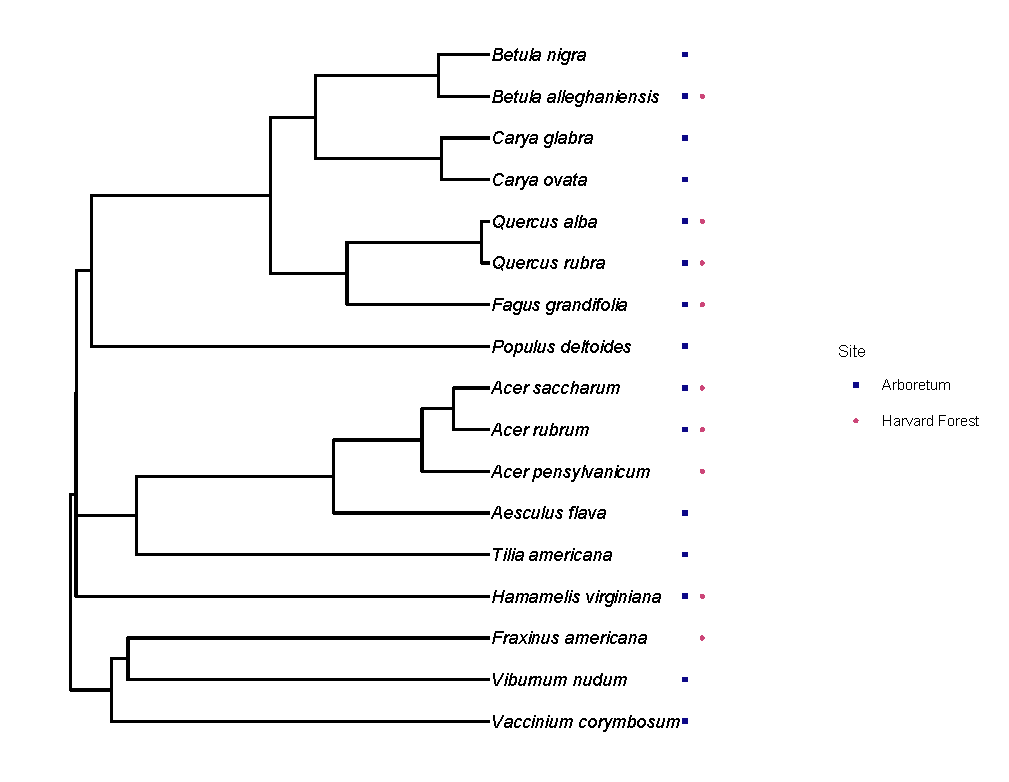
\includegraphics[width=12cm]{..//phylodata/microtree_hfandts.pdf}
  -\caption{Phylogeny indicating species across the two sites}\label{fig:phylo}
  -\end{center}
  -\end{figure}}


% latex table generated in R 4.0.3 by xtable 1.8-4 package
% Mon May  3 18:20:31 2021
\begin{table}[ht]
\centering
\caption{\textbf{Estimates from urban simulations}. We present posterior means, as well as 50\% and 95\% uncertainty intervals from models in which the predictors have been standardized so that they are comparable.} 
\label{tab:urban}
\begingroup\footnotesize
\begin{tabular}{|p{0.11\textwidth}|p{0.06\textwidth}p{0.06\textwidth}p{0.06\textwidth}p{0.06\textwidth}p{0.06\textwidth}|}
  \hline
 & mean & 25\% & 75\% & 2.5\% & 97.5\% \\ 
  \hline
$\mu_{\alpha}$ & 307.40 & 303.75 & 310.96 & 296.83 & 318.49 \\ 
  $\mu_{site}$ & 20.67 & 20.08 & 21.25 & 19.01 & 22.30 \\ 
  $\mu_{method}$ & 0.23 & -0.35 & 0.80 & -1.49 & 1.97 \\ 
  $\mu_{sitexmethod}$ & -0.36 & -1.19 & 0.38 & -2.57 & 2.01 \\ 
  $\sigma_{site}$ & 1.18 & 0.56 & 1.65 & 0.06 & 2.93 \\ 
  $\sigma_{method}$ & 1.09 & 0.46 & 1.57 & 0.05 & 2.84 \\ 
  $\sigma_{sitexmethod}$ & 0.75 & 0.28 & 1.06 & 0.02 & 2.28 \\ 
  $\sigma_{\alpha}$ & 21.49 & 18.37 & 23.99 & 14.82 & 31.44 \\ 
  $\sigma_{y}$ & 15.57 & 15.44 & 15.69 & 15.18 & 15.97 \\ 
   \hline
$N_{sp}$ & 15.00 &  &  &  &  \\ 
   \hline
\end{tabular}
\endgroup
\end{table}



% latex table generated in R 4.0.3 by xtable 1.8-4 package
% Mon May  3 18:20:31 2021
\begin{table}[ht]
\centering
\caption{\textbf{Estimates from microclimate simulations}. We present posterior means, as well as 50\% and 95\% uncertainty intervals from models in which the predictors have been standardized so that they are comparable.} 
\label{tab:micros}
\begingroup\footnotesize
\begin{tabular}{|p{0.11\textwidth}|p{0.06\textwidth}p{0.06\textwidth}p{0.06\textwidth}p{0.06\textwidth}p{0.06\textwidth}|}
  \hline
 & mean & 25\% & 75\% & 2.5\% & 97.5\% \\ 
  \hline
$\mu_{\alpha}$ & 322.94 & 318.50 & 327.45 & 310.33 & 335.58 \\ 
  $\mu_{site}$ & -0.32 & -0.91 & 0.30 & -2.11 & 1.42 \\ 
  $\mu_{method}$ & -6.78 & -8.07 & -5.50 & -10.55 & -3.07 \\ 
  $\mu_{sitexmethod}$ & 1.05 & 0.26 & 1.85 & -1.33 & 3.38 \\ 
  $\sigma_{site}$ & 1.14 & 0.47 & 1.65 & 0.06 & 3.12 \\ 
  $\sigma_{method}$ & 6.82 & 5.63 & 7.72 & 4.26 & 10.92 \\ 
  $\sigma_{sitexmethod}$ & 1.23 & 0.46 & 1.77 & 0.04 & 3.60 \\ 
  $\sigma_{\alpha}$ & 24.85 & 21.32 & 27.48 & 17.17 & 36.72 \\ 
  $\sigma_{y}$ & 16.73 & 16.59 & 16.87 & 16.32 & 17.14 \\ 
   \hline
$N_{sp}$ & 15.00 &  &  &  &  \\ 
   \hline
\end{tabular}
\endgroup
\end{table}



\begin{figure}[H]
      \centering
      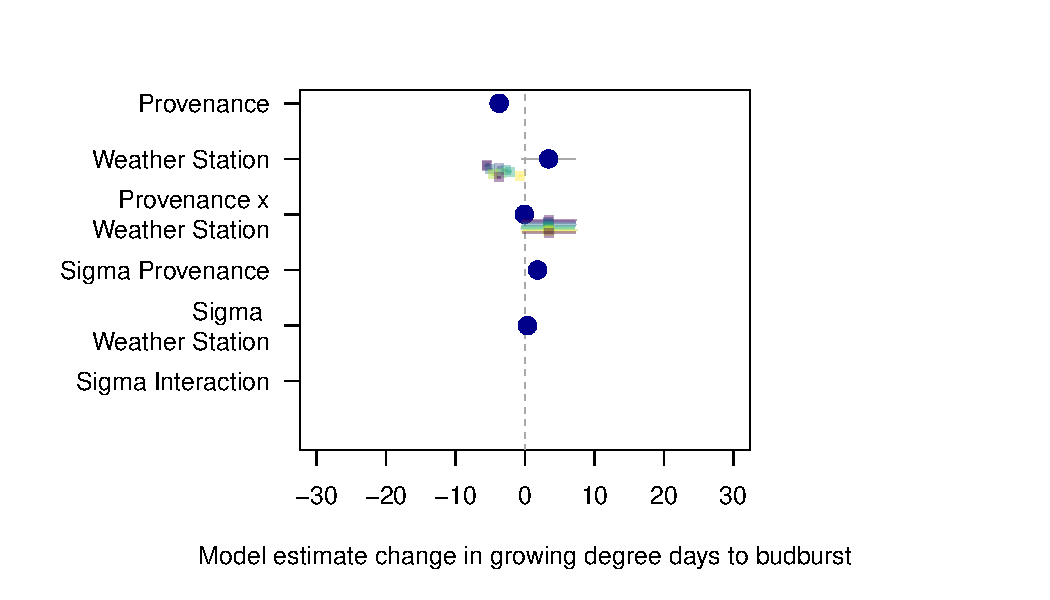
\includegraphics[height=7cm, width=11cm]{..//analyses/figures/muplot_prov.pdf}
      \label{fig:muplotprovsims}
\caption{ Using simulated data to test provenance latitude, we show (a) the effects of provenance latitude and climate data method (weather station data as `1' or hobo logger data as `0') on simulated growing degree days (GDDs) until budburst. More positive values indicate more GDDs are required for budburst whereas more negative values suggest fewer GDDs are required. Dots and thin lines show means and 90\% uncertainty intervals and thicker lines show 50\% uncertainty intervals. See Table \ref{tab:prov} for full model output. }
\label{fig:provsims}
\end{figure}

% latex table generated in R 4.0.3 by xtable 1.8-4 package
% Mon May  3 18:20:31 2021
\begin{table}[ht]
\centering
\caption{\textbf{Estimates from provenance latitude simulations}. We present posterior means, as well as 50\% and 95\% uncertainty intervals from models in which the predictors have been standardized so that they are comparable.} 
\label{tab:prov}
\begingroup\footnotesize
\begin{tabular}{|p{0.11\textwidth}|p{0.06\textwidth}p{0.06\textwidth}p{0.06\textwidth}p{0.06\textwidth}p{0.06\textwidth}|}
  \hline
 & mean & 25\% & 75\% & 2.5\% & 97.5\% \\ 
  \hline
$\mu_{\alpha}$ & 307.61 & 304.40 & 310.79 & 296.64 & 318.14 \\ 
  $\mu_{site}$ & -4.80 & -5.38 & -4.22 & -6.47 & -3.05 \\ 
  $\mu_{method}$ & -0.29 & -0.69 & 0.11 & -1.50 & 0.90 \\ 
  $\mu_{sitexmethod}$ & -0.54 & -1.41 & 0.32 & -3.03 & 1.96 \\ 
  $\sigma_{site}$ & 0.94 & 0.39 & 1.35 & 0.04 & 2.61 \\ 
  $\sigma_{method}$ & 0.77 & 0.33 & 1.09 & 0.03 & 2.13 \\ 
  $\sigma_{sitexmethod}$ & 1.58 & 0.72 & 2.23 & 0.08 & 4.08 \\ 
  $\sigma_{\alpha}$ & 20.54 & 17.57 & 22.71 & 14.07 & 30.22 \\ 
  $\sigma_{y}$ & 15.57 & 15.43 & 15.71 & 15.19 & 15.96 \\ 
   \hline
$N_{sp}$ & 15.00 &  &  &  &  \\ 
   \hline
\end{tabular}
\endgroup
\end{table}



% latex table generated in R 4.0.3 by xtable 1.8-4 package
% Mon May  3 18:20:31 2021
\begin{table}[ht]
\centering
\caption{\textbf{Estimates from noisy weather station simulations}. We present posterior means, as well as 50\% and 95\% uncertainty intervals from models in which the predictors have been standardized so that they are comparable.} 
\label{tab:noisyws}
\begingroup\footnotesize
\begin{tabular}{|p{0.11\textwidth}|p{0.06\textwidth}p{0.06\textwidth}p{0.06\textwidth}p{0.06\textwidth}p{0.06\textwidth}|}
  \hline
 & mean & 25\% & 75\% & 2.5\% & 97.5\% \\ 
  \hline
$\mu_{\alpha}$ & 307.45 & 303.99 & 310.89 & 297.13 & 318.19 \\ 
  $\mu_{site}$ & 0.07 & -0.50 & 0.66 & -1.54 & 1.69 \\ 
  $\mu_{method}$ & 4.93 & 2.35 & 7.60 & -3.09 & 12.52 \\ 
  $\mu_{sitexmethod}$ & -0.39 & -1.16 & 0.36 & -2.81 & 1.84 \\ 
  $\sigma_{site}$ & 0.68 & 0.26 & 0.98 & 0.02 & 1.93 \\ 
  $\sigma_{method}$ & 14.63 & 12.37 & 16.33 & 9.81 & 22.36 \\ 
  $\sigma_{sitexmethod}$ & 0.86 & 0.33 & 1.23 & 0.03 & 2.59 \\ 
  $\sigma_{\alpha}$ & 21.79 & 18.43 & 24.37 & 14.47 & 33.19 \\ 
  $\sigma_{y}$ & 15.55 & 15.42 & 15.67 & 15.16 & 15.95 \\ 
   \hline
$N_{sp}$ & 15.00 &  &  &  &  \\ 
   \hline
\end{tabular}
\endgroup
\end{table}



% latex table generated in R 4.0.3 by xtable 1.8-4 package
% Mon May  3 18:20:31 2021
\begin{table}[ht]
\centering
\caption{\textbf{Estimates from noisy hobo logger simulations}. We present posterior means, as well as 50\% and 95\% uncertainty intervals from models in which the predictors have been standardized so that they are comparable.} 
\label{tab:noisyhobo}
\begingroup\footnotesize
\begin{tabular}{|p{0.11\textwidth}|p{0.06\textwidth}p{0.06\textwidth}p{0.06\textwidth}p{0.06\textwidth}p{0.06\textwidth}|}
  \hline
 & mean & 25\% & 75\% & 2.5\% & 97.5\% \\ 
  \hline
$\mu_{\alpha}$ & 316.41 & 311.01 & 321.54 & 299.27 & 333.71 \\ 
  $\mu_{site}$ & -1.20 & -1.78 & -0.62 & -2.89 & 0.51 \\ 
  $\mu_{method}$ & -6.41 & -9.15 & -3.68 & -14.64 & 1.86 \\ 
  $\mu_{sitexmethod}$ & 2.15 & 1.36 & 2.91 & -0.10 & 4.47 \\ 
  $\sigma_{site}$ & 1.00 & 0.42 & 1.43 & 0.03 & 2.73 \\ 
  $\sigma_{method}$ & 15.14 & 12.73 & 17.02 & 10.11 & 23.17 \\ 
  $\sigma_{sitexmethod}$ & 1.20 & 0.48 & 1.70 & 0.04 & 3.31 \\ 
  $\sigma_{\alpha}$ & 31.87 & 27.47 & 35.30 & 22.11 & 46.96 \\ 
  $\sigma_{y}$ & 15.05 & 14.91 & 15.19 & 14.67 & 15.46 \\ 
   \hline
$N_{sp}$ & 15.00 &  &  &  &  \\ 
   \hline
\end{tabular}
\endgroup
\end{table}





% latex table generated in R 4.0.3 by xtable 1.8-4 package
% Mon May  3 18:20:31 2021
\begin{table}[ht]
\centering
\caption{\textbf{Estimates from real data}. We present posterior means, as well as 50\% and 95\% uncertainty intervals from models in which the predictors have been standardized so that they are comparable.} 
\label{tab:real}
\begingroup\footnotesize
\begin{tabular}{|p{0.11\textwidth}|p{0.06\textwidth}p{0.06\textwidth}p{0.06\textwidth}p{0.06\textwidth}p{0.06\textwidth}|}
  \hline
 & mean & 25\% & 75\% & 2.5\% & 97.5\% \\ 
  \hline
$\mu_{\alpha}$ & 424.96 & 413.29 & 437.11 & 387.75 & 458.74 \\ 
  $\mu_{site}$ & -31.66 & -39.63 & -23.74 & -54.08 & -9.28 \\ 
  $\mu_{method}$ & -0.50 & -7.29 & 6.22 & -19.96 & 20.45 \\ 
  $\mu_{sitexmethod}$ & -40.35 & -48.17 & -32.56 & -63.08 & -17.80 \\ 
  $\sigma_{site}$ & 21.46 & 11.46 & 29.44 & 1.25 & 49.34 \\ 
  $\sigma_{method}$ & 17.09 & 7.80 & 24.21 & 0.88 & 43.70 \\ 
  $\sigma_{sitexmethod}$ & 25.62 & 16.26 & 33.80 & 2.66 & 52.91 \\ 
  $\sigma_{\alpha}$ & 62.95 & 53.51 & 71.16 & 40.91 & 93.12 \\ 
  $\sigma_{y}$ & 71.54 & 69.73 & 73.28 & 66.63 & 76.75 \\ 
   \hline
$N_{sp}$ & 18.00 &  &  &  &  \\ 
   \hline
\end{tabular}
\endgroup
\end{table}



\begin{figure}[H]
      \centering
      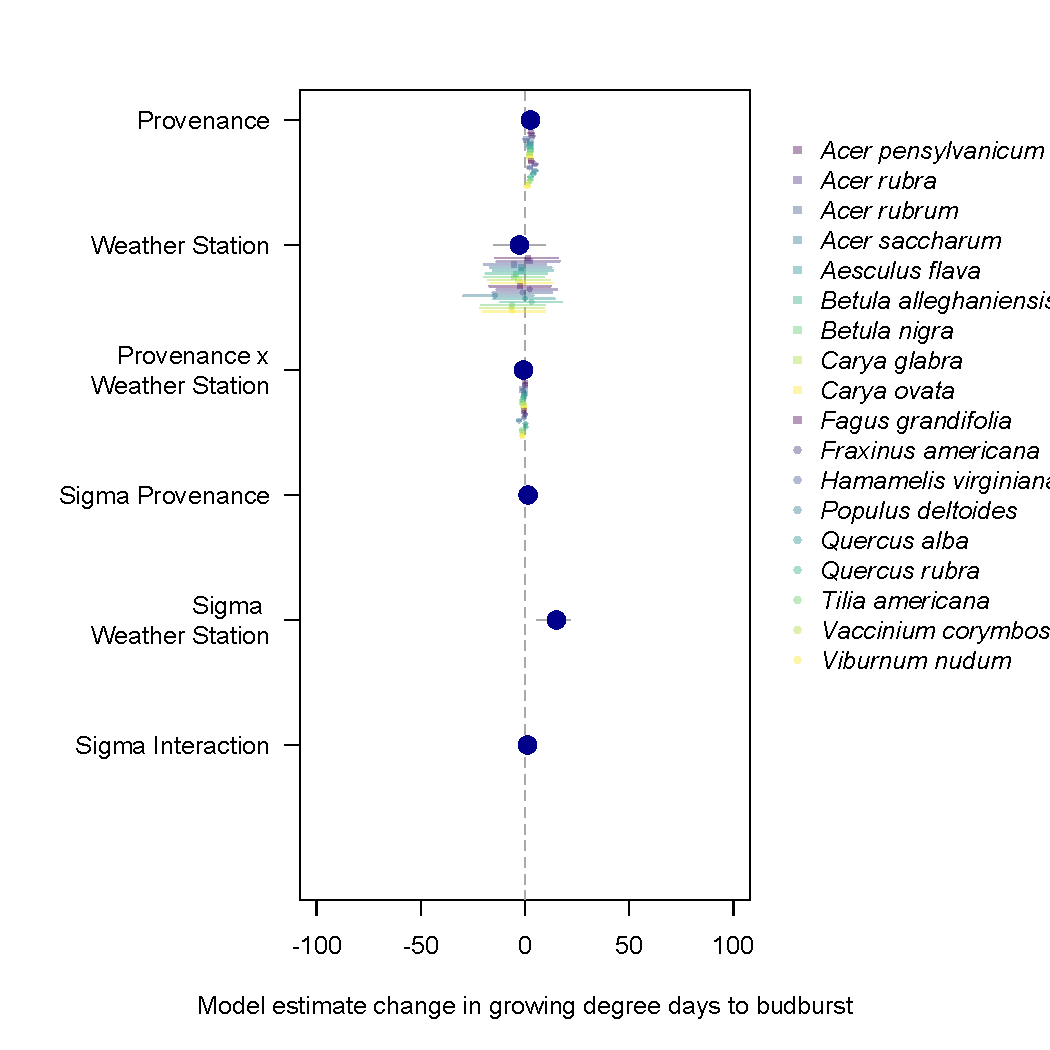
\includegraphics[height=7cm, width=11cm]{..//analyses/figures/muplot_prov_real.pdf}
      \label{fig:muplotprov}
\caption{ Using real data to test provenance latitude, we show the effects of provenance latitude and climate data method (weather station data as `1' or hobo logger data as `0') on simulated growing degree days (GDDs) until budburst. More positive values indicate more GDDs are required for budburst whereas more negative values suggest fewer GDDs are required. Dots and thin lines show means and 90\% uncertainty intervals and thicker lines show 50\% uncertainty intervals. See Table \\ref{tab:provreal} for full model output.}
\label{fig:prov}
\end{figure}

% latex table generated in R 4.0.3 by xtable 1.8-4 package
% Mon May  3 18:20:31 2021
\begin{table}[ht]
\centering
\caption{\textbf{Estimates from provenance latitude}. We present posterior means, as well as 50\% and 95\% uncertainty intervals from models in which the predictors have been standardized so that they are comparable.} 
\label{tab:provreal}
\begingroup\footnotesize
\begin{tabular}{|p{0.11\textwidth}|p{0.06\textwidth}p{0.06\textwidth}p{0.06\textwidth}p{0.06\textwidth}p{0.06\textwidth}|}
  \hline
 & mean & 25\% & 75\% & 2.5\% & 97.5\% \\ 
  \hline
$\mu_{\alpha}$ & 394.32 & 382.18 & 406.76 & 356.00 & 430.30 \\ 
  $\mu_{site}$ & 18.15 & 11.68 & 24.64 & -0.64 & 38.01 \\ 
  $\mu_{method}$ & -8.46 & -12.51 & -4.27 & -20.81 & 3.92 \\ 
  $\mu_{sitexmethod}$ & -3.53 & -9.65 & 2.73 & -22.29 & 16.00 \\ 
  $\sigma_{site}$ & 15.43 & 7.31 & 21.21 & 0.73 & 40.78 \\ 
  $\sigma_{method}$ & 8.45 & 3.47 & 12.23 & 0.36 & 23.60 \\ 
  $\sigma_{sitexmethod}$ & 13.69 & 6.11 & 19.41 & 0.49 & 37.55 \\ 
  $\sigma_{\alpha}$ & 71.80 & 62.26 & 79.36 & 50.01 & 102.94 \\ 
  $\sigma_{y}$ & 78.76 & 76.81 & 80.70 & 73.40 & 84.53 \\ 
   \hline
$N_{sp}$ & 18.00 &  &  &  &  \\ 
   \hline
\end{tabular}
\endgroup
\end{table}


  
\begin{figure}[H]
    \centering
    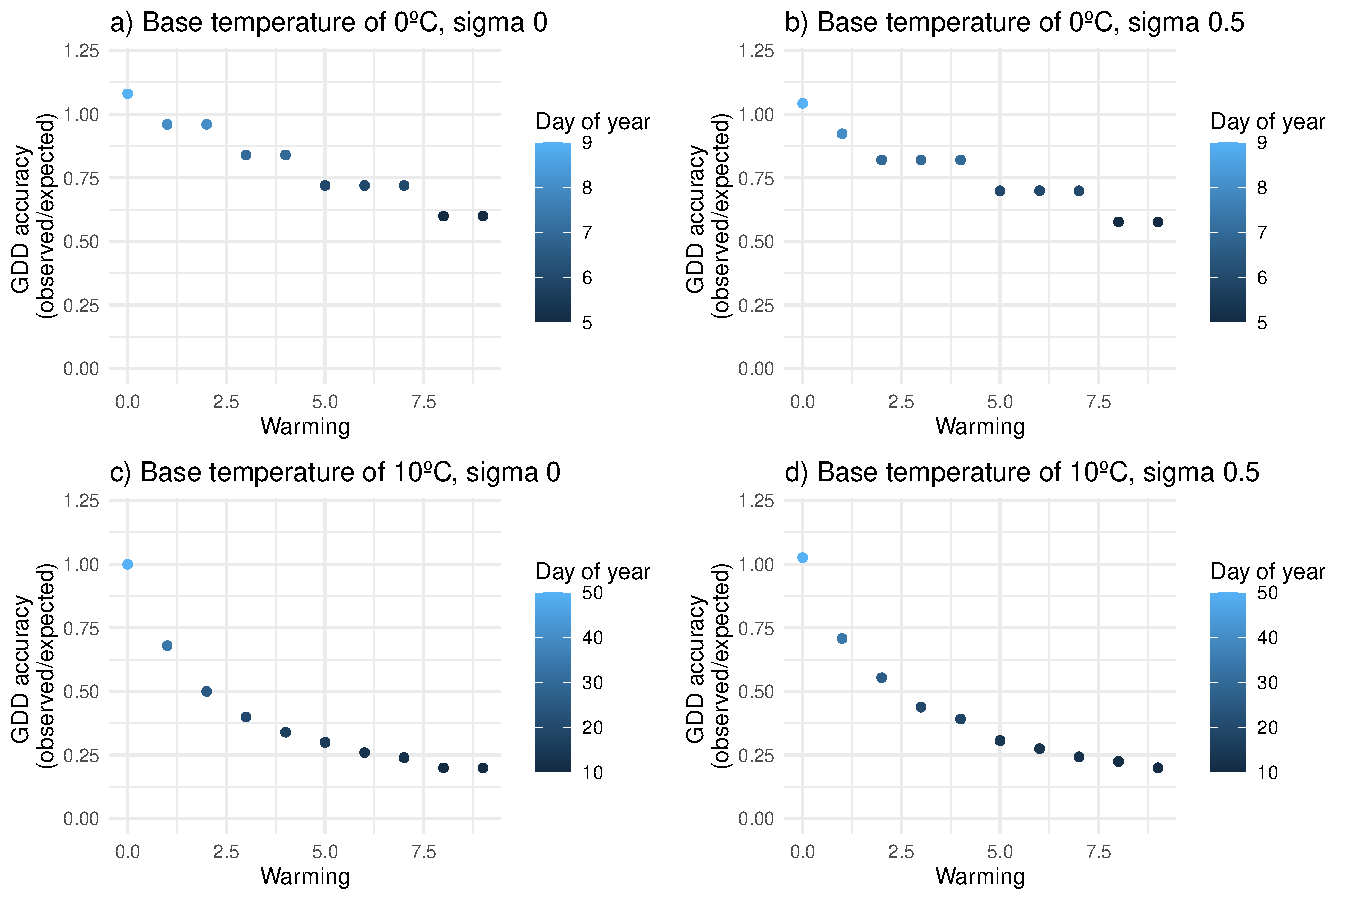
\includegraphics[height=8cm, width=12cm]{..//analyses/figures/gddratio_warming.pdf}
\caption{Using simulated data, we show how GDD measurement accuracy changes with warming (i.e., from 0$^{\circ}$C to 10$^{\circ}$C) using a base temperature of (a) 0$^{\circ}$C and a sigma of 0$^{\circ}$C, (b) 0$^{\circ}$C and a sigma of 0.5$^{\circ}$C, (c) 10$^{\circ}$C and a sigma of 0$^{\circ}$C and (d) 10$^{\circ}$C and a sigma of 0.5^{\circ}$C. GDD accuracy is measured as the observed GDD divided by the expected GDD. }
\label{fig:warming}
\end{figure}



\end{document}
